%% Le Rapporteur --- VLDB-style research paper (PVLDB / acmart sigconf).
%% Compile: tectonic paper/main.tex   (tectonic fetches acmart on first run)
%% Camera-ready: replace the \vldb* placeholders below and switch to the
%% official PVLDB template if submitting.
\documentclass[sigconf, nonacm]{acmart}

% ---- PVLDB front-matter placeholders (fill for a real submission) ----
\newcommand\vldbdoi{XX.XX/XXX.XX}
\newcommand\vldbpages{XXX-XXX}
\newcommand\vldbvolume{XX}
\newcommand\vldbissue{X}
\newcommand\vldbyear{2026}
\newcommand\vldbauthors{W. Dor\'e and F. Amat}
\newcommand\vldbtitle{Le Rapporteur}
\newcommand\vldbavailabilityurl{https://github.com/wilfred-dore/hackathon-assemblee-2026}
\newcommand\vldbpagestyle{plain}

% Draft: no ACM reference block / CCS / conference furniture.
\settopmatter{printacmref=false, printccs=false, printfolios=true}
\pagestyle{plain}

\usepackage{booktabs}
\usepackage{listings}
\usepackage{tikz}
\usetikzlibrary{arrows.meta, positioning, fit, backgrounds, shapes.geometric}
\usepackage{xcolor}

\definecolor{lrblue}{HTML}{000091}
\definecolor{lrred}{HTML}{E1000F}
\definecolor{lrgray}{HTML}{555555}

\lstdefinestyle{lr}{
  basicstyle=\ttfamily\footnotesize,
  breaklines=true,
  columns=fullflexible,
  keepspaces=true,
  frame=single,
  framesep=4pt,
  xleftmargin=3pt,
  showstringspaces=false,
  commentstyle=\color{lrgray}\itshape,
  keywordstyle=\color{lrblue}\bfseries,
}

\begin{document}

\title{Le Rapporteur: Fail-Closed, Database-Verified Legal
Question Answering on Sovereign Hardware}

\author{Wilfred Dor\'e}
\affiliation{%
  \institution{\'Equipe Le Rapporteur}
  \city{Hackathon Assembl\'ee nationale}
  \country{France}}
\email{wilfred.dore@telecom-paristech.org}

\author{Fran\c{c}ois Amat}
\affiliation{%
  \institution{\'Equipe Le Rapporteur}
  \city{Hackathon Assembl\'ee nationale}
  \country{France}}
\email{contact@famat.me}

\renewcommand{\shortauthors}{Dor\'e and Amat}

\begin{abstract}
Large language models (LLMs) answer legal questions fluently, but they
routinely \emph{invent} statutory citations that look plausible and are
wrong. In law, a confident wrong answer is worse than no answer. We present
\emph{Le Rapporteur}, a legal question-answering system built on one
non-negotiable rule: \textbf{no verifiable source, no answer}. The model
generates a draft; every cited article (e.g., \emph{article L.\,3121-27 du
Code du travail}) is extracted and checked, one by one, against a live legal
database (Canutes, a mirror of the French Légifrance corpus); if a single
citation cannot be resolved to an \emph{in-force} article, the system returns
an explicit refusal rather than a fabrication. We describe (i) the
database-centric verifier and the query engineering required to check
citations at interactive latency over a 253-table corpus without
full-table scans, (ii) a reusable trust service exposing the verifier over
HTTP and the Model Context Protocol (MCP) so any agent can fact-check an
LLM's output, (iii) a hardware-\emph{sovereign} serving layer that runs the
identical pipeline on non-NVIDIA silicon (Qualcomm Cloud~AI~100, live) via a
single OpenAI-compatible indirection, and (iv) an executable, jurist-readable
trust specification in Gherkin where one fabricated article breaks the build.
We report qualitative evidence---including a live model that cited a
plausible but wrong article, caught by the verifier---and discuss the gap
between \emph{existence} checking and \emph{semantic} correctness, which
motivates our grounding roadmap.
\end{abstract}

\keywords{legal NLP, retrieval, hallucination, fact verification, LLM serving,
sovereignty, Model Context Protocol, open government data}

\maketitle

%% PVLDB reference format (compact; fill placeholders for camera-ready).
\begingroup\small\noindent\raggedright
\textbf{Draft --- PVLDB-style formatting.}\
Artifacts: \url{https://github.com/wilfred-dore/hackathon-assemblee-2026}.
\endgroup

\section{Introduction}
Citizens increasingly ask general-purpose LLMs questions of law. The models
answer in fluent, authoritative prose---and sometimes cite articles that do
not exist, or that exist but say something else. Unlike open-domain chit-chat,
the legal domain has an asymmetric cost structure: a plausible-sounding but
fabricated citation actively \emph{misleads}, and is worse than an admission
of ignorance. Hallucination in natural language generation is by now
well documented~\cite{ji2023hallucination}, and retrieval augmentation is the
standard mitigation~\cite{lewis2020rag}; yet grounding a generation in
retrieved passages \emph{reduces} but does not \emph{guarantee} the absence of
invented references.

\emph{Le Rapporteur} takes a deliberately conservative stance suited to law.
The system is organized around a single invariant---\textbf{no verifiable
source, no answer}---enforced not by prompt engineering but by a
post-generation verification stage that is \emph{fail-closed}: any doubt,
network error, or unresolved reference collapses to an explicit refusal
(``Je ne trouve pas de texte applicable.'', \emph{I find no applicable
text.}). The design is a defense in depth: the model may draft freely, but
nothing reaches the user unless each citation resolves to a real, in-force
article in an authoritative database.

\paragraph{Contributions.}
\begin{itemize}
  \item A \textbf{fail-closed pipeline} for legal QA (\emph{generate,
  extract, verify, source-or-refuse}) whose trust guarantee is a property of
  the \emph{system}, not of the model (\S\ref{sec:overview}).
  \item A \textbf{database-centric citation verifier} over the Canutes/Légifrance
  corpus, and the query engineering (index-friendly citation normalization,
  state-aware selection of the in-force version) that makes per-citation
  checking feasible at interactive latency over a large, irregular schema
  without full-table regular-expression scans (\S\ref{sec:verify}).
  \item A \textbf{reusable trust service}: the verifier is exposed over HTTP
  (\texttt{/verify}) and as a Model Context Protocol (MCP) server, so any
  third-party agent can fact-check the citations in an arbitrary LLM output
  (\S\ref{sec:service}).
  \item A \textbf{hardware-sovereign serving layer}: an OpenAI-compatible
  indirection lets the identical pipeline run on non-NVIDIA accelerators; we
  demonstrate it live on a Qualcomm Cloud~AI~100 and target AMD via a portable
  runtime (\S\ref{sec:sovereign}).
  \item An \textbf{executable trust specification} in Gherkin, readable and
  auditable by a jurist, in which a single fabricated article fails the build
  (\S\ref{sec:bdd}).
\end{itemize}

We are candid throughout about what is \emph{proven} versus \emph{envisioned};
this project was built under hackathon constraints and we mark roadmap items
explicitly.

\section{Background and Problem}
\label{sec:background}

\paragraph{French legal open data.}
French statutory law is published as open data by the DILA through
Légifrance~\cite{legifrance}. Our verification target is \emph{Canutes}, a
PostgreSQL corpus mirroring this data. Two properties shape the engineering.
First, the schema is large and irregular: on the order of $253$ tables with
cryptic names, of which a public PostgREST~\cite{postgrest} endpoint exposes
only three---insufficient for verification. Second, articles are versioned:
the same numbered article (e.g., \emph{L.\,3121-27}) has multiple rows over
time, and only the \texttt{VIGUEUR} (in-force) version is authoritative for a
citizen's question. Verification must therefore be \emph{state-aware}.

\paragraph{Why not RAG alone.}
Retrieval-augmented generation~\cite{lewis2020rag} conditions the model on
retrieved passages and improves faithfulness, but the model can still
paraphrase a real passage into a wrong article number, or cite a neighbor.
Our position is that grounding and \emph{post-hoc verification} are
complementary: grounding improves the draft; verification provides the
guarantee. This paper focuses on the guarantee.

\section{System Overview}
\label{sec:overview}

Figure~\ref{fig:pipeline} shows the pipeline. A citizen question is sent to a
sovereign LLM. The draft answer is parsed for legal citations of the canonical
French form \emph{``article $\langle$num$\rangle$ du $\langle$code$\rangle$''}
using a normalization-tolerant extractor. Each extracted citation is verified
independently against the legal database. The answer is released
\emph{only if} the set of citations is non-empty and \emph{every} citation
resolves to an in-force article; otherwise the system refuses. This
\emph{fail-closed} disjunction is the whole point: the guarantee does not
depend on the model behaving well.

\begin{figure}[t]
\centering
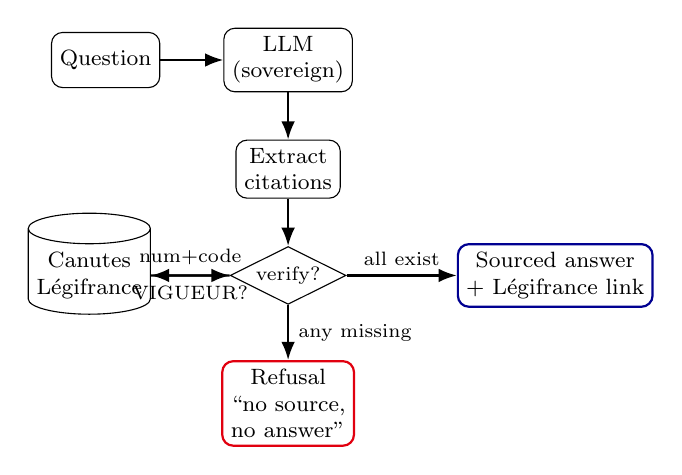
\begin{tikzpicture}[
  node distance=6mm and 8mm,
  box/.style={draw, rounded corners, align=center, font=\footnotesize,
              minimum height=7mm, inner sep=3pt},
  db/.style={draw, cylinder, shape border rotate=90, aspect=0.25,
             align=center, font=\footnotesize, inner sep=3pt},
  dec/.style={draw, diamond, aspect=2, align=center, font=\scriptsize, inner sep=1pt},
  ok/.style={draw=lrblue, thick, rounded corners, align=center, font=\footnotesize, inner sep=3pt},
  no/.style={draw=lrred, thick, rounded corners, align=center, font=\footnotesize, inner sep=3pt},
  a/.style={-{Latex}, thick}]
  \node[box] (q) {Question};
  \node[box, right=of q] (g) {LLM\\(sovereign)};
  \node[box, below=of g] (e) {Extract\\citations};
  \node[dec, below=of e] (v) {verify?};
  \node[db, left=of v, xshift=-2mm] (db) {Canutes\\Légifrance};
  \node[ok, right=of v, xshift=6mm] (r) {Sourced answer\\+ Légifrance link};
  \node[no, below=of v, yshift=-1mm] (x) {Refusal\\``no source,\\no answer''};
  \draw[a] (q) -- (g);
  \draw[a] (g) -- (e);
  \draw[a] (e) -- (v);
  \draw[a] (v) -- (db) node[midway, above, font=\scriptsize] {num+code};
  \draw[a] (db) -- (v) node[midway, below, font=\scriptsize] {VIGUEUR?};
  \draw[a] (v) -- (r) node[midway, above, font=\scriptsize] {all exist};
  \draw[a] (v) -- (x) node[midway, right, font=\scriptsize] {any missing};
\end{tikzpicture}
\caption{The fail-closed pipeline: \emph{generate, extract, verify,
source-or-refuse}. The trust guarantee is enforced at the verification
diamond, independently of the model.}
\label{fig:pipeline}
\end{figure}

\section{Citation Verification over a Legal Database}
\label{sec:verify}

The verifier answers a deceptively simple query: \emph{does article
$\langle$num$\rangle$ of $\langle$code$\rangle$ exist and is it in force?} Doing
this at interactive latency over Canutes required care.

\paragraph{Index-friendly citation matching.}
Légifrance encodes article numbers inconsistently (e.g., \texttt{L3121-27},
\texttt{L.\,3121-27}, \texttt{L. 3121-27}). A naive predicate
(\texttt{num \textasciitilde{} '.*3121-27.*'}) forces a sequential scan and a
regular-expression match over the whole \texttt{legifrance.article} table,
which in our environment hit a statement timeout. Instead, we expand the
citation into a small, closed set of \emph{exact} string variants and match
with equality against the (indexable) \texttt{num} column:

\begin{lstlisting}[style=lr, language=SQL]
-- variants = {"L. 3121-27", "L.3121-27", "L3121-27", ...}
SELECT id, num, data
FROM   legifrance.article
WHERE  num = ANY(%s)          -- equality, index-friendly
  AND  data::text ILIKE %s    -- code name appears in the article JSON
LIMIT  200;
\end{lstlisting}

\paragraph{Code disambiguation and accents.}
The code name (e.g., \emph{Code du travail}) is matched by \texttt{ILIKE}
against the article's JSON payload, then re-checked in Python with an
accent-insensitive normalization (Postgres \texttt{ILIKE} is not
accent-folding). This two-stage filter keeps the SQL cheap while remaining
correct on inputs such as \emph{Code de la s\'ecurit\'e sociale}.

\paragraph{State-aware selection.}
Among the surviving rows we prefer the \texttt{VIGUEUR} (in-force) version;
if present, we return its canonical \texttt{LEGIARTI} identifier, from which we
build a real, clickable Légifrance URL, plus a short text excerpt. If no row
matches the code, the verifier returns \texttt{exists=false}, which the
pipeline treats as a refusal trigger. Crucially, \emph{every failure mode maps
to ``not verified''}: this is what makes the layer fail-closed.

\paragraph{Offline determinism.}
For demos and tests without network access, a mock verifier answers from a
small local set of articles known to be in force. The same code path yields a
deterministic, reproducible refusal for a fabricated article---essential for
the executable specification of \S\ref{sec:bdd}.

\section{A Reusable Trust Service}
\label{sec:service}

Rather than a monolithic chatbot, Le Rapporteur exposes its trust layer as a
service others can call. Over HTTP:
\begin{itemize}
  \item \texttt{POST /answer} --- ask a question, receive a sourced answer or a
  refusal, with each citation annotated \{\,exists, url, excerpt\,\} and,
  under a live backend, latency/throughput metrics;
  \item \texttt{POST /verify} --- submit \emph{arbitrary} text (e.g., another
  LLM's output) and receive, per citation, whether it is real, plus aggregate
  flags (\texttt{n\_invented}, \texttt{trustworthy}).
\end{itemize}
\texttt{/verify} is the key integration point: any citizen platform or
parliamentary tool can detect invented legal citations in a third-party model's
output without adopting our model.

The same two capabilities---\texttt{repondre\_question} and
\texttt{verifier\_article}---are also exposed as a \textbf{Model Context
Protocol} server~\cite{mcp2024} (JSON-RPC 2.0 over streamable HTTP). Le
Rapporteur is thus a \emph{provider}, not merely a consumer, of verified legal
knowledge: an agent such as a general assistant can call it as a tool. We
verified interoperability by driving our own MCP client against this server.

\section{Hardware-Sovereign Serving}
\label{sec:sovereign}

Serving an open-weight LLM is, in practice, often equivalent to depending on a
single vendor's stack (CUDA/NVIDIA). For a system whose remit is national law,
that coupling is itself a sovereignty risk. Our serving layer is a thin
\emph{OpenAI-compatible} indirection: switching silicon is switching three
environment variables (\texttt{LLM\_BASE\_URL}, \texttt{LLM\_API\_KEY},
\texttt{LLM\_MODEL}); the pipeline is unchanged.

Table~\ref{tab:backends} states, honestly, what runs where. We demonstrate the
pipeline \emph{live} on a Qualcomm Cloud~AI~100 inference
accelerator~\cite{qualcommcloudai100} (Llama-3.1-8B), a dedicated
inference silicon whose value proposition is operations-per-watt rather than
raw training throughput. We target AMD via a portable inference
runtime~\cite{modularmax2024}; European accelerators are stated as vision, not
measurement. We report real latency and tokens/s; we deliberately do
\emph{not} report a fabricated energy figure, citing only that dedicated
inference silicon is designed for high throughput-per-watt.

\begin{table}[t]
\centering
\caption{Serving backends and honest status. The pipeline is identical across
rows; only the OpenAI-compatible endpoint changes.}
\label{tab:backends}
\small
\begin{tabular}{@{}lll@{}}
\toprule
Backend & Silicon & Status \\
\midrule
Qualcomm Cloud AI 100 & Qualcomm & \textbf{live, proven} \\
Modular MAX & AMD Instinct & target (runtime supports it) \\
Modular MAX & NVIDIA & backward compatibility \\
Self-hosted (open weights) & NVIDIA (cloud) & fallback \\
VSora / Axelera & EU/FR & vision (no access) \\
\bottomrule
\end{tabular}
\end{table}

\section{An Executable Trust Specification}
\label{sec:bdd}

The anti-hallucination guarantee is not a slogan; it is encoded as
behavior-driven tests in Gherkin~\cite{gherkin}, in French, so that a lawyer
(not only an engineer) can read and audit them. The suite runs on every
change; \emph{a single fabricated article turns the build red}.

\begin{lstlisting}[style=lr]
Scenario: No invented citation
  Given a citizen question "Ai-je droit a la prime de Noel ?"
  When the system answers
  Then the answer must be an explicit refusal
  And no article absent from the sources may be
      presented as verified
\end{lstlisting}

Three scenarios cover the invariant: a verified citation must be sourced; a
question that elicits a fabricated article (the ``Christmas bonus'', for which
the model invents \emph{article L.\,4321-7}) must be refused; and a question
with no verifiable source must be refused. Turning trust into a red/green test
makes the property continuously checkable rather than merely asserted.

\section{Qualitative Evaluation and Observations}
\label{sec:eval}

This is a hackathon system; we report observations, not a benchmark. The
executable specification passes ($3/3$ scenarios) in the deterministic offline
mode. Under the live Qualcomm backend we observed the intended failure being
caught in the wild: asked for the legal working week, the model answered with
\emph{article L.\,3132-2} (which exists, but concerns weekly rest) instead of
the correct \emph{L.\,3121-27}; the verifier flagged the mismatch and the
system refused rather than emit the plausible-but-wrong citation. This is
precisely the class of error a fluent model produces and a database check
catches.

\section{Limitations and Future Work}
\label{sec:limits}

\paragraph{Existence is not semantics.}
Our verifier checks that a cited article \emph{exists} and is \emph{in force};
it does not yet check that the article's \emph{content} supports the claim.
We observed the model cite an article that exists but is off-topic
(\emph{L.\,2122-4}); such a citation passes an existence check. Closing this
gap requires semantic verification (entailment between the article text and the
answer's claim).

\paragraph{Grounding.}
The current system \emph{generates then verifies}; it does not yet retrieve
before generating. The planned grounding is \emph{lexical}, not vectorial: a
full-text search (via a metadata-aware SQL tool, or Postgres
\texttt{to\_tsvector}) returning top-$k$ passages that condition generation.
The obstacle is not a vector store but an efficient full-text \emph{index}
over a very large article table---indexing the entire corpus is the real wall,
so we would scope to a sub-corpus first.

\paragraph{Model and hardware.}
Mistral is not served by our live Qualcomm endpoint (Llama-3.1-8B only); a
Mistral deployment via the portable runtime on AMD is future work, as is a
kernel-level (Mojo) hot-path benchmark for perf/watt claims.

\section{Related Work}
\label{sec:related}

Hallucination in generation is surveyed by Ji et al.~\cite{ji2023hallucination};
retrieval augmentation~\cite{lewis2020rag} is the dominant mitigation. Our
contribution is orthogonal and complementary: a \emph{fail-closed, database-backed
verification} layer specialized to a versioned legal corpus, exposed as a
reusable service over MCP~\cite{mcp2024}. On the systems side, the work is a
small study in making per-citation checks cheap over an irregular open-government
schema, and in decoupling a trust pipeline from the serving
silicon~\cite{modularmax2024, qualcommcloudai100}.

\section{Conclusion}
In law, refusing is a feature. Le Rapporteur enforces ``no verifiable source,
no answer'' by verifying every citation against a live legal database and
failing closed on any doubt, exposes that verification as a reusable service,
and runs unchanged on sovereign, non-NVIDIA silicon. The guarantee is a
property of the system and is continuously tested. The path from
\emph{existence} checking to \emph{semantic} verification, and from
post-hoc checking to grounded generation, is our next step.

\bibliographystyle{ACM-Reference-Format}
\bibliography{references}

\end{document}
